\subsection{A formulation for contact}

The problem of a beam in contact with a rigid wall can be described by a further augmented Lagrangian $\Tilde{L}$, \cite{alart1991}.

\begin{equation}\label{eq:L_constraint}
    \Tilde{L} = L - k g(q) \Lambda_c + \frac{p}{2} g(q)^2 - \frac{1}{2p} \left( dist\left( k \Lambda_c - pg(q), \mathbb{R}^+ \right) \right)^2
\end{equation}

Here, $k$ is a scaling factor, $g$ is the gap function w.r.t. the wall, $\Lambda_c$ is a Lagrange multiplier, and $p$ is a positive penalty coefficient. One can recognise a Lagrange multiplier term, a penalty term and distance term, where $\xi=k \Lambda_c - pg$ is the augmented Lagrange multiplier. The latter can represent two possible scenarios, i.e. for $\xi<0$ the contact forces are not active, while for $\xi>0$ the contact is activated. \\
In this particular case study, we are interested in investigating the elastica in a narrow environment as in Figure~\ref{fig:ESR10_contact} where two rigid straight walls are implemented.

\begin{figure}[!ht]
    \centering
    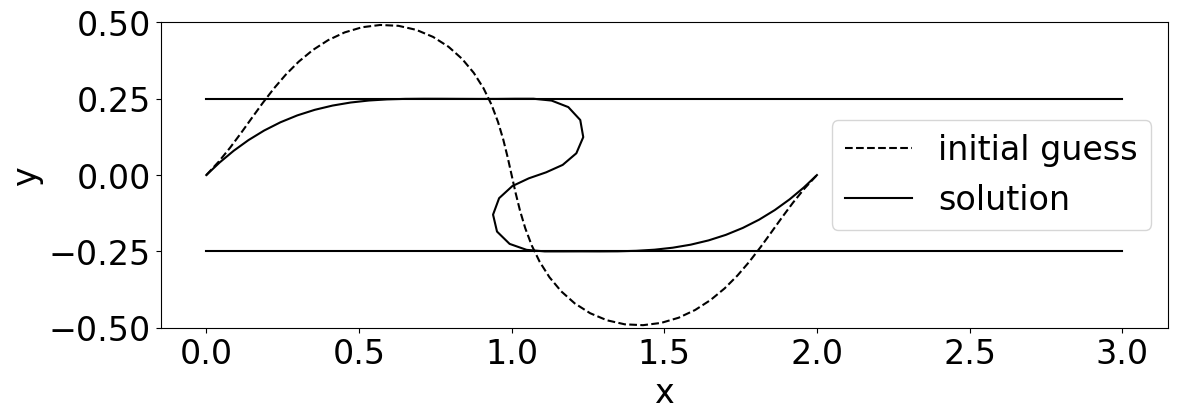
\includegraphics[width=7.5cm]{figures/contact_bw.png}
    \caption{Case study: beam in a narrow straight tube}
    \label{fig:ESR10_contact}
\end{figure}




